\chapter{Marco Te\'orico}
\section{El Lenguaje}
En un contexto general el lenguaje es un sistema de comunicaci\'on que todo ser vivo 
utiliza para intercambiar informaci\'on con sus semejantes mediante el uso de
s\'imbolos, se\~nales y sonidos percibidos por los \'organos sensoriales. \\

El principal tipo lenguaje utilizado por el ser humano es el \emph{Lenguaje Natural}, 
adem\'as se han desarrollado otros tipos de lenguajes para su comunicaci\'on como ser 
el lenguaje braille y el lenguaje de se\~nas, que son utilizados en ausencia de 
capacidades para utilizar un lenguaje natural. \\

Otros tipos de lenguajes existentes son los \emph{lenguajes formales}, que
son construcci\'ones artificiales, donde los s\'imbolos y reglas para unir los mismos
est\'an formalmente especificados, los lenguajes de programaci\'on utilizados en 
inform\'atica son un ejemplo de lenguaje formal.

\section{Lenguaje Natural}
Las capacidades humanas de comunicaci\'on se basan en el uso de signos ling\"uisticos
que se componen por un concepto (\emph{significado}) y una imagen ac\'ustica
(\emph{significante}), cuando estos signos se asocian a una sintaxis generan  una
\emph{lengua natural}, el uso de estas lenguas describen un lenguaje natural. \\

Los idiomas como ser el espa\~nol o el ingles, al contar con un conjunto de signos
(\emph{alfabeto}) y reglas sint\'acticas (\emph{gram\'atica}) propias para cada uno,
representan lenguajes naturales.

\subsection{Alfabeto}
Es el conjunto de simbolos utilizados en un idioma para representar estructuras del
lenguaje como las palabras.


\subsection{Gram\'atica}
Es el conjunto de reglas que gobiernan la composici\'on de las palabras dentro de un
lenguaje natural.

\section{La Palabra}
La Palabra es la unidad m\'inima con significado que se puede pronunciar de manera
aislada (evidencia fonol\'ogica)\cite{HOET09}. La rama de la ling\"uistica que estudia
la composici\'on y estructura interna de las palabras es la morfolog\'ia.


\subsection{Clasificaci\'on de las palabras}
La clasificaci\'on de las palabras se puede hacer en funci\'on de diferentes criterios:
categor\'ia gramatical, estructura interna, acentuaci\'on y n\'umero de s\'ilabas; para
los fines del presente trabajo se tomara en cuenta la clasificaci\'on seg\'un su
categor\'ia gramatical tambi\'en conocido como \emph{parte de la oraci\'on}
(part-of-speech en ingl\'es), es la siguiente:
\begin{description}[leftmargin=0cm]
	\item[Sustantivo] Son palabras cuyo referentes son entidades fijas, todo aquello a 
	lo que le damos un nombre: \emph{perro}, \emph{Pablo}, etc.
	\item[Verbo] Son palabras que expresan acci\'on o movimiento, presentan formas
	conjugadas: \emph{correr}, \emph{preguntar}, etc.
	\item[Adjetivo] Son palabras que califican al sustantivo para completarlo expresando
	caracter\'isticas y propiedades: \emph{grande}, \emph{r\'apido}, etc.
	\item[Adverbio] Son palabras que sirven para modificar a un verbo, adjetivo u otro
	adverbio: \emph{muy}, \emph{poco}, \emph{adelante}, etc.
	\item[Determinante] Son palabras que precisan un sustantivo, transform\'andolo de
	abstracto a concreto: \emph{el}, \emph{la}, \emph{un}, etc.
	\item[Preposici\'on] Son palabras invariantes que ligan el nombre con un verbo:
	\emph{a}, \emph{en}, \emph{de}, etc.
	\item[Conjunci\'on] Son palabras que un a otras: \emph{y}, \emph{pero}, etc.
	\item[Pronombre] Son palabras cuyo referente no es fijo sino que se determina
	en relaci\'on con otras: \emph{yo}, \emph{alg\'un}, \emph{m\'io}, etc.
	\item[Interjecci\'on] Son palabras que expresan alguna impresi\'on s\'ubita o
	sentimiento profundo: \emph{Ay!}, \emph{Eh!}, etc.
\end{description}

\section{Procesamiento del Lenguaje Natural}
El Procesamiento del Lenguaje Natural (PLN) es un campo de la inform\'atica y la 
ling\"uistica concerniente con la interacci\'on entre computadoras y lenguajes
humanos. \\

La interacci\'on se produce con la \emph{generaci\'on} de lenguaje legible por humanos
a partir de datos procesados y la \emph{comprensi\'on} del lenguaje humano para su
representaci\'on formal.

\section{Palabras clave}
Las palabras clave se definen como una secuencia de una o mas palabras que idealmente
proveen una representaci\'on compacta de la esencia del contenido de un 
documento \cite{REC10}. \\

Las palabras clave se utilizan para catalogar e indexar material bibliogr\'afico,
su identificaci\'on es una de las tareas principales en el procesamiento de texto. \\

La asignaci\'on manual de palabras claves de calidad es costosa, consume tiempo y es
propensa a error, por lo tanto se han propuesto varios m\'etodos para su seleccio\'on
autom\'atica.

\subsection{M\'etodos de selecci\'on de palabras clave}
Los m\'etodos de selecci\'on de palabras claves se dividen en cuatro categor\'ias:
estad\'isticas simples, ling\"uisticos, aprendizaje autom\'atico y otros \cite{ZWW08}.
\begin{description}[leftmargin=0cm]
	\item[Enfoques estad\'isticos] Son los mas simples, no necesitan datos previos,
	la informaci\'on estad\'istica de las palabras pueden ser usadas para identificar
	las palabras clave en un documento.
	\item[Enfoques ling\"uisticos] Utilizan las caracter\'isticas l\'exicas y
	sint\'acticas de las palabras, sentencias y documentos.
	\item[Enfoques de aprendizaje autom\'atico] Se basan en el aprendizaje supervisado
	a partir de datos de ejemplo para generar un modelo y aplicarlo a nuevos
	documentos.
	\item[Otros enfoques] Combinan los m\'etodos anteriormente mencionados o utilizan
	conocimiento heur\'istico.
\end{description}

\section{Modelo TextRank}
Es un m\'odelo de puntuaci\'on basado en grafos para el procesamiento de
texto \cite{RMPT04}, que es utilizado para la extracci\'on de palabras claves
y sentencias mediante algoritmos de puntuaci\'on basados en grafos.
% TODO: Completar este concepto

\subsection{Algoritmos de puntuaci\'on basados en grafos}
Son algoritmos que se utilizan para obtener valores significativos
(\emph{calificaci\'on}) de los nodos en un grafo. \\

Existen varios algoritmos de puntuaci\'on: \emph{PageRank} de Google,
\emph{HITS} de Kleinberg, \emph{Positional Function} de Herings \cite{RM04}. \\

A continuaci\'on se describe el algoritmo PageRank.

\subsubsection{Algoritmo PageRank}
\begin{figure}
	\centering
		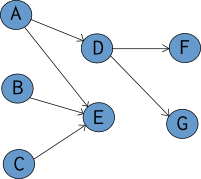
\includegraphics[]{recursos/img/grafoDirigido.png}
		\caption {Grafo dirigido}
\end{figure}

Dado $G=(V,E)$ un grafo dirigido, con un conjunto de v\'ertices $V$ y un conjunto
de arcos $E$, donde $E$ es un subconjunto de $V x V$, llamamos $In(V_i)$ al
conjunto de v\'ertices que apuntan a $V_i$ (predecesores),  en la Figura 2.1
$In(E)=\{A,B,C\}$, y $Out(V_i)$ al conjunto de v\'ertices que son apuntados por $(V_i)$
(sucesores), en la Figura 2.1 $Out(D)=\{F,G\}$ . El puntaje del v\'ertice $V_i$ 
esta dado por \cite{SBLP98}:

\begin{equation}
	S(V_i) = (1 - d) + d * \sum_{V_j\in In(V_i)}{\frac{1}{|Out(V_j)|}S(V_j)}
\end{equation}

donde $d$ es un factor de amortiguaci\'on que toma valores comprendidos entre
0 y 1, que expresa la probabilidad de avanzar de un v\'ertice a otro de manera
aleatoria, generalmente tiene el valor de 0.85 \cite{SBLP98}.

\subsection{Aplicaci\'on en la extracci\'on de palabras claves}
El grafo es construido de la siguiente manera: se seleccionan palabras  para 
conformar los v\'ertices, si existe una relaci\'on de \emph{co-ocurrencia} entre 
las palabras seleccionadas, se a\~nade un nodo entre ellas. \\

Las palabras seleccionadas son aquellas que pasan por un filtro sint\'actico, el cual
selecciona solo las unidades l\'exicas pertenecientes a un conjunto definido de tipos
de palabras. \\

Se pueden seleccionar todos los tipos de palabras, o un conjunto restringido a verbos
y sustantivos, se presentan mejores resultados con el conjunto de verbos y
adjetivos \cite{RMPT04} .
